\documentclass[11pt]{article}
    \usepackage{caption}
    \usepackage{graphicx}
    \usepackage{mathtools}
    \usepackage{bookmark}
    \graphicspath{ {img/} }
    \setlength{\parindent}{0pt}
    \DeclareCaptionType{equ}[][]
    \usepackage[svgnames]{xcolor}
    
    \newcommand*{\plogo}{\fbox{$\mathcal{BM}$}}
        
    \usepackage{PTSerif}
    
    \begin{document} 
        
    \begin{titlepage}
    
        \raggedleft
        
        \vspace*{\baselineskip}
        
        {\Large Bryan Melanson}
        
        \vspace*{0.167\textheight}
        
        \textbf{\LARGE How to Not Fail}\\[\baselineskip]
        
        {\textcolor{Red}{\Huge Digital System Design}}\\[\baselineskip]
        
        {\Large \textit{While never going to class}}
        
        \vfill
        
        {\large Computer Engineering 2020 ~~\plogo}
        
        \vspace*{3\baselineskip}
    
    \end{titlepage}

    \pagebreak
    
%%%%%%%%%%%%%%%%%%%%%%%%%%%%%%%%%%%%%%%%%%%%%%%%%
    \pdfbookmark[section]{\contentsname}{toc}

    \tableofcontents

    \pagebreak
%%%%%%%%%%%%%%%%%%%%%%%%%%%%%%%%%%%%%%%%%%%%%%%%%
    \section{Implementation Technology}
    \subsection{VLSI}
    "Very Large-Scale Integration" refers to circuit devices that contain thousands to millions of transistors. \\ 
    \textbf{Pros}
    \begin{enumerate}
        \item Complete control overall aspects of circuit implementation
        \item Can optimize for speed, area, power as needed
        \item Allows you to achieve highest device performance
        \item Cost effective for large volume designs
        \item Facilitates mixed-signal design
    \end{enumerate}
    \textbf{Cons}
    \begin{enumerate}
        \item Manufacturing is costly
        \item Mistakes are costly
        \item Verification process is long and thorough
        \item Design process is slow - long time to market
        \item Device functionality is static - no way to add system features
    \end{enumerate}

    \subsection{ASIC}
    "Application Specific Integrated Circuit" same manufacturing as VLSI, with reduced design time, made of predefined components. These libraries are accessed with a HDL based design and synthesis process, and then mapped to an implementation in the target technology. \\ 
    \textbf{Pros}
    \begin{enumerate}
        \item Faster design time than VLSI
        \item Some ability to optimize for speed, area, power as needed
        \item Allows you to achieve good device performance
        \item Can be cost effective for large volume designs
        \item Faster testing and verification than VLSI
    \end{enumerate}
    \textbf{Cons}
    \begin{enumerate}
        \item Manufacturing is costly
        \item Mistakes are costly
        \item Testing and verification is slow
        \item Design and manufacturing is slow - long time to market
        \item Once manufactured, device functionality is static - no way to add system features
    \end{enumerate}

    \subsection{Programmable Logic}
    \subsubsection{Simple Programmable Logic Devices}
    Programmable logic forms were factory programmable such as ROMs and MPGAs (mask programmable gate arrays). The connection between these devices must be designed by the designer, which shortens design time compared to VLSI and ASIC.
    \subsubsection{ROMs/LUTs}
    ROMs were intended as memory devices (such as cartridges) but could be used for logic functions. ROMs can store a truth table to implement combinational logic. Each ROM has $n$ address lines and $m$ data outputs.
    \subsubsection{PLAs/PLDs}
    Programmable Logic Arrays (PLA) are based on the notion that any logic function is a combination of product terms OR'd together. \\
    \begin{center}
        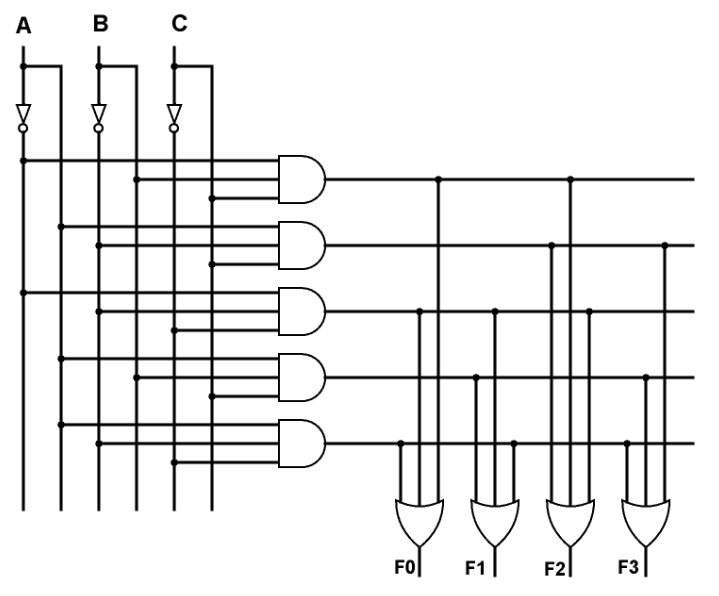
\includegraphics[width=300 px]{pla} 
    \end{center}   
    \subsection{FPGAs}
    Field Programmable Gate Arrays are flexible programmable logic for larger designs. Complicated to program, but offer large capacities and flexibility. 
    \begin{enumerate}
        \item Programmable I/O blocks - Pin configuration
        \item Programmable Logic blocks - LUTs, AND-OR, multiplexers, etc.
        \item Programmable Routing Resources - Routing between the pins and blocks
    \end{enumerate}


    \textbf{Pros}
    \begin{enumerate}
        \item Faster design time than VLSI
        \item Reduced cost of design errors
        \item Flexibility for new requirements
        \item Cost effective when low number of devices
    \end{enumerate}
    \textbf{Cons}
    \begin{enumerate}
        \item Lower logic density (unused elements take up space)
        \item Higher power consumption
        \item Not applicable to all designs - floating point
    \end{enumerate}
    \pagebreak

%%%%%%%%%%%%%%%%%%%%%%%%%%%%%%%%%%%%%%%%%%%%%%%%%
    \section{Intro to VHDL}
    \textbf{VHDL} ("VHSIC" (Very High Speed Integrated Circuit) Hardwre Description Language) describes digital circuits but can be used to generate circuits automatically (\textit{synthesis}). This facilitates top down design, and provides reusable elements and mature design practices. This can reduce the cost of prototyping complicated systems. \\
    
    \subsection{Timing}
    \verb#C <= A and B after 5 ns# \\ 

    The \textbf{after} will ensure A and B are assigned to C 5 ns after being evaluated. \\ 

    \verb#C <= reject 3 ns inertial A and B after 5 ns# \\ 

    If a pulse occurs for less than 3 ns, it will be rejected. If longer than the rejection time, it will be propogated after a 5 ns delay. Inertial delay is the default delay assumed by VHDL.\\
    
    \verb#C <= transport A after 10 ns# \\ 

    Transport will delay the signals without rejecting.

    \subsection{Data Types}
    \begin{enumerate}
        \item bit - 0, or 1
        \item bit vector - an array of 0, 1
        \item std logic - 0, 1, X, U, etc
        \item std logic vector - array of std logic
    \end{enumerate}

    \subsection{VHDL Modules}
    \textbf{Entity} similar to a function prototype. Describes port inpus and outputs.\\ 

    \textbf{Architecture} is a description of the internals. \\
    
    \begin{center}
        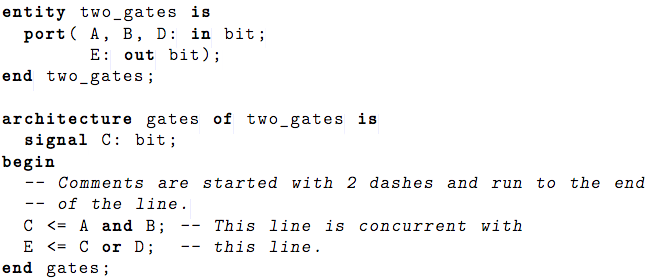
\includegraphics[width=300 px]{vhdl} 
    \end{center}  

    The devices can be reused in separate files by declaring it as a component and instantiating each element individually, assigning pins.

    \begin{center}
        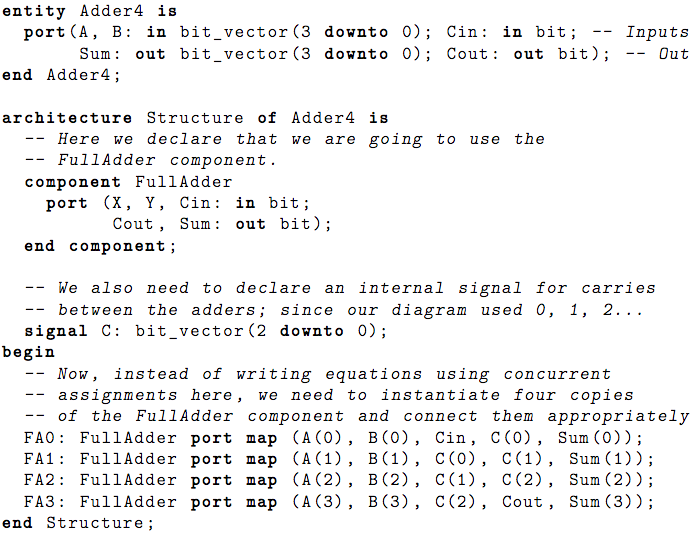
\includegraphics[width=300 px]{vhdl2} 
    \end{center}  

    \subsection{Sequential Statements}

    The \textbf{process} statement will monitor a signal using a sensitivity list and trigger a sequence of lines to be completed in order. 

    \begin{center}
        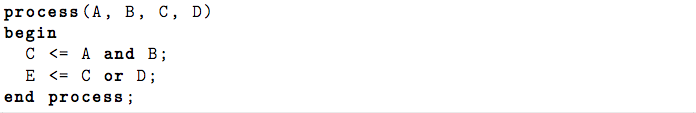
\includegraphics[width=300 px]{process} 
    \end{center} 

    \subsection{Flip Flops}

    \begin{center}
        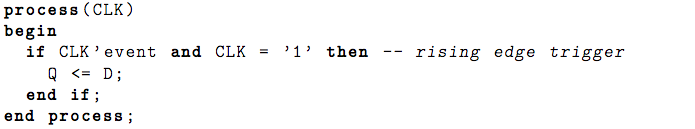
\includegraphics[width=300 px]{flipflops} 
    \end{center} 

    \subsection{Conditional Assignments}

    \begin{center}
        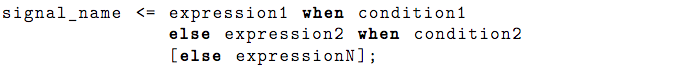
\includegraphics[width=300 px]{condition} 
    \end{center} 

    \begin{center}
        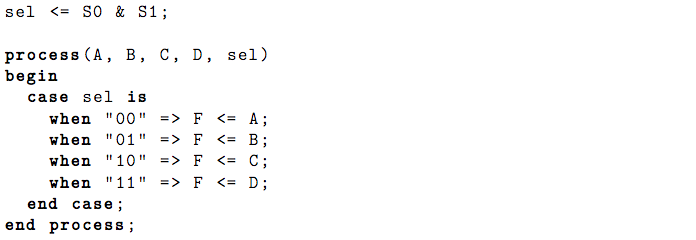
\includegraphics[width=300 px]{case} 
    \end{center} 

    \subsection{User Defined Types} 
    
    \begin{center}
        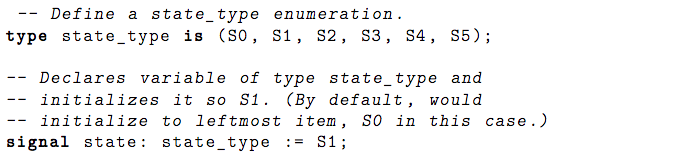
\includegraphics[width=300 px]{types} 
    \end{center} 

    \begin{center}
        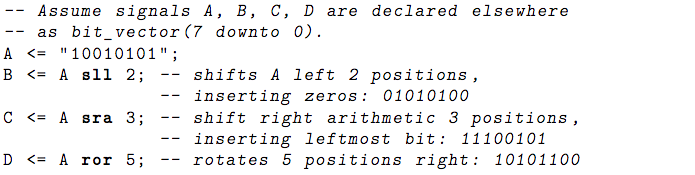
\includegraphics[width=300 px]{shifts} 
    \end{center} 

    \pagebreak
%%%%%%%%%%%%%%%%%%%%%%%%%%%%%%%%%%%%%%%%%%%%%%%%%
    \section{Advanced Design}
    \subsection{Logic Minimization}
    \begin{center}
        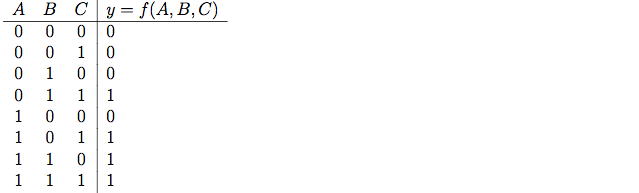
\includegraphics[width=300 px]{logic} 
    \end{center} 
    $y - A'BC + AB'C + ABC' + ABC$ can be reduced to \textbf{minterms}. \\ 

    $\sum m(3,5,6,7)$ \\
    
    This is known as the Standard Sum of Products form - this can also incorporate Don't-Care: \\
    
    $\sum m(3,5,6,7) + \sum d(0,3)$

    \subsection{Quine McCluskey Method}

    This reduces the SSOP form to a minimum sum of products by eliminating as many literals as possible to produce prime implicants, and then createing a chart of implicants to be OR'd to implement the original function. \\subsection{
        
    Recall $XY + XY' = X$ - use this to combine minterms if they differ in one minterm. Terms are then represented as binary, for example $AB'CD' = 1010$, so $AB'CD' + AB'CD = AB'C$ or $101-$.

    \begin{center}
        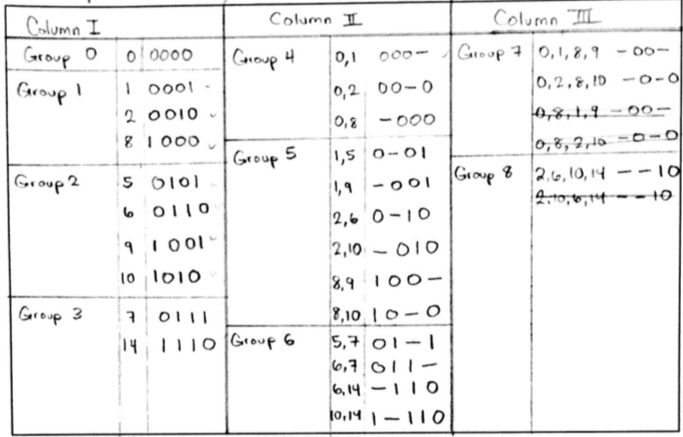
\includegraphics[width=300 px]{quine} 
    \end{center} 

    The numbers which don't reduce to the following column or are redundant are \textit{prime implicants}. In this case, the prime implicants are $0-01$, $01-1$, $011-$, $-00-$, $-0-0$, and $--10$.

    \begin{center}
        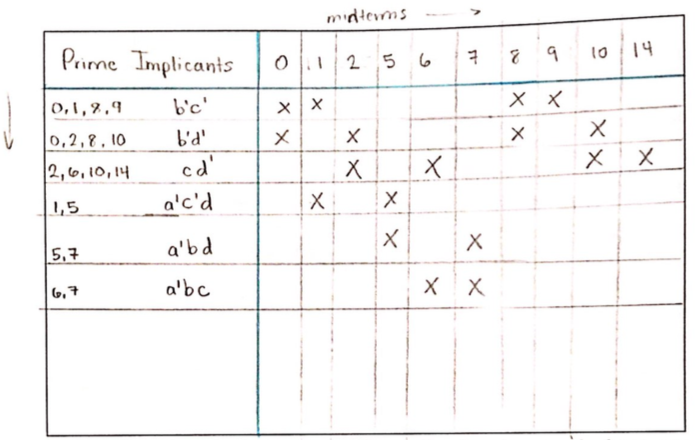
\includegraphics[width=300 px]{implicants} 
    \end{center} 

    \begin{center}
        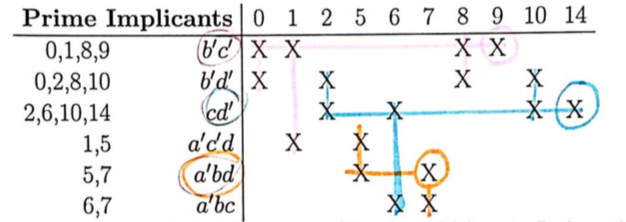
\includegraphics[width=300 px]{implicants2} 
    \end{center} 

    Choose the values with a single X in its column, then draw a horizontal line through the row. Any intersections, draw a vertical line. Continue until all X are crossed out, choosing values which will cover off as much as possible.

    \pagebreak
%%%%%%%%%%%%%%%%%%%%%%%%%%%%%%%%%%%%%%%%%%%%%%%%%
    \section{Hazards and Testing}
    \subsection{Hazards in Combinational Circuits}
    \subsubsection{Static 1 Hazard}
    If a circuit goes 0 when it should have been 1
    \subsubsection{Static 0 Hazard}
    A circuit goes 1 when it should be constant 0
    \subsubsection{Dynamic Hazard}
    When the circuit should transition from 0 to 1 or 1 to 0, but transitions three or more times

    \begin{center}
        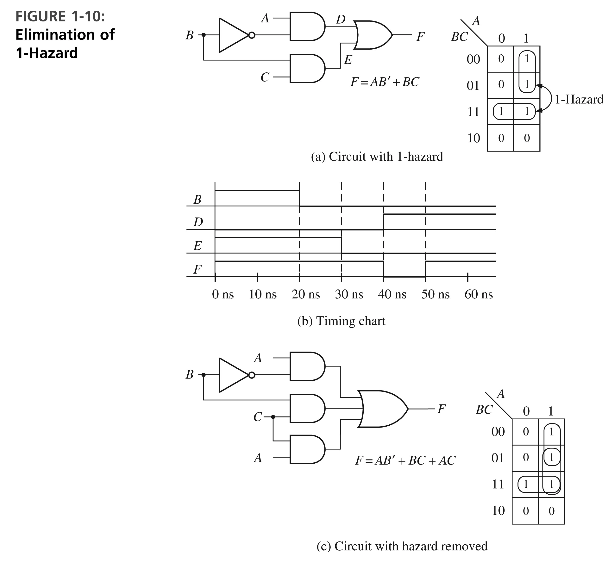
\includegraphics[width=300 px]{hazard} 
    \end{center} 

    Select inputs to test specific port errors:

    \begin{center}
        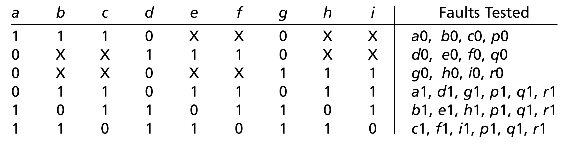
\includegraphics[width=300 px]{test} 
    \end{center}   

    \subsection{Scan Testing}

    

    \pagebreak
%%%%%%%%%%%%%%%%%%%%%%%%%%%%%%%%%%%%%%%%%%%%%%%%%
    \section{Memory and Arithmetic}
    \pagebreak
%%%%%%%%%%%%%%%%%%%%%%%%%%%%%%%%%%%%%%%%%%%%%%%%%
    \section{More VHDL}
    \pagebreak
%%%%%%%%%%%%%%%%%%%%%%%%%%%%%%%%%%%%%%%%%%%%%%%%%
    \section{System Design}
    \subsection{AMBA/AXI}
    \textbf{AMBA} is a protocol created by ARM for components designed for other companies. This is an open standard on-chip interconnect for connection and management of blocks in a System-On-Chip. \\
    
    AMBA has four interface protocols, \textit{AXI} (Advanced Extemsible Interface), \textit{AHB} (Advanced High Performance Bus), \textit{APB} (Advanced Peripheral Bus), and \textit{ATB} (Advanced Trace Bus). \\
    
    \textbf{AXI4-Lite} is a subset of AXI4 used for simpler control register style interfaces. All transactions are burst legnths of 1, data accesses are the same size and width as the data bus, and exclusive access is not supported. 

    \begin{center}
        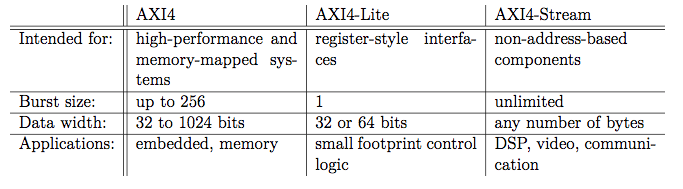
\includegraphics[width=300 px]{axi} 
    \end{center}    

    \textbf{Channel} is a collection of signals associated to a VALID signal. \\
    
    \textbf{Interface} is a collection of 1 or more channels that expose an IP's core function. An IP core can have multiple interfaces. \\

    \textbf{Bus} is a multiple bit signal (may be part of an interface or channel, but distinct). \\

    \textbf{Transfer} is a single clock cycle where information is communicated qualified by a VALID handshake. \\

    \textbf{Transaction} is a complete communication operator across a channel composed of one or more transfers. \\

    \textbf{Burst} is a transaction consisting of more than 1 transfer. \\

    An AXI4 handshake is as follows:

    \begin{enumerate}
        \item Master asserts a VALID when data is available
        \item Slave asserts READY if able to accept
        \item Date is transferred when VALID and READY
        \item If the transaction has more than 1 transfer, next data is sent, otherwise VALID is removed
        \item If slave cannot accept, READY is removed to pause
    \end{enumerate}

    \begin{center}
        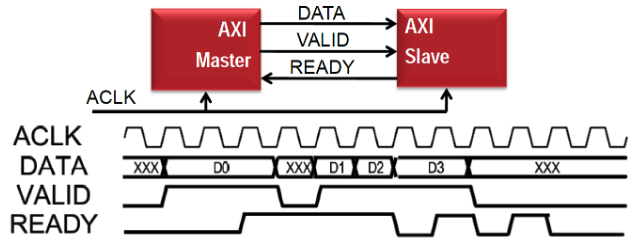
\includegraphics[width=300 px]{handshake} 
    \end{center}    

    AXI4 and variants all have 5 basic signalling channels:

    \begin{enumerate}
        \item Read address
        \item Read data
        \item Write address
        \item Write data
        \item Write response (Slave to Master)
    \end{enumerate}

    \begin{center}
        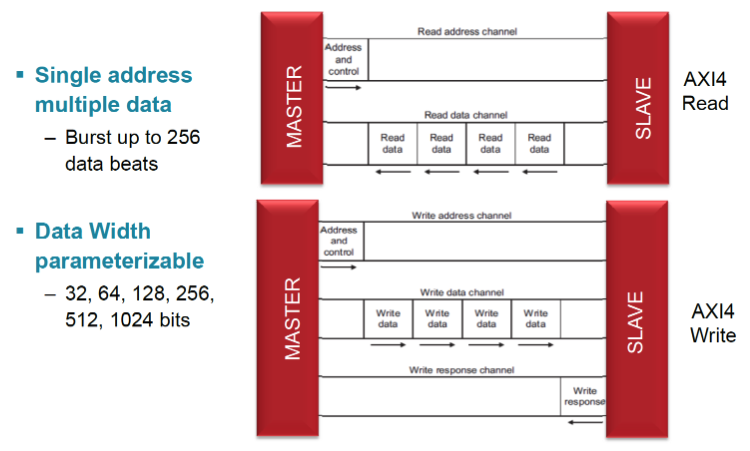
\includegraphics[width=300 px]{axi-sm} 
    \end{center}   

    For AXI-Lite, only 1 data tranfer per transaction.

    \begin{center}
        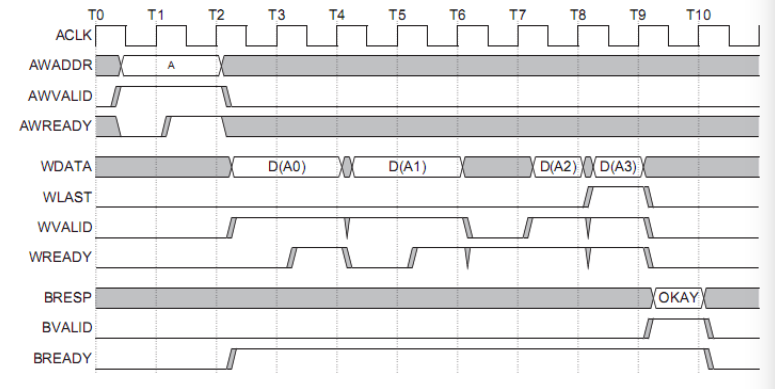
\includegraphics[width=300 px]{axi_read} 
    \end{center}   

    \begin{center}
        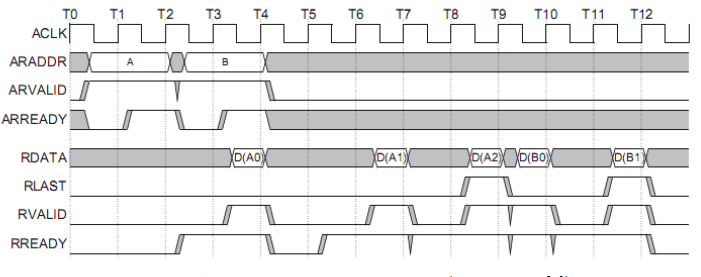
\includegraphics[width=300 px]{axi_write} 
    \end{center}   

    \textbf{Write Address Channel (AXI4-Lite)}

    AWVALID - The address write valid signal (master to slave) \\
    AWREADY - The address write ready signal (slave to master)\\
    AWADDR - The target write address \\
    AWPROT - The protection type specifying privilege and security level \\

    \textbf{Write Data Channel (AXI4-Lite)}

    WVALID - The data write valid signal (master to slave)\\
    WREADY - The data write ready signal (slave to master)\\
    WDATA - The n-bit write data \\
    WSTRB - The write strobe lines indicate with bytes hold valid data (1 bti for each 8 bit data) \\

    \textbf{Write Response Channel (AXI4-Lite)}

    BVALID - The write response valid signal (slave to master) \\
    BREADY - The write reponse ready signal (master to slave) \\
    BRESP - Write reponse indicating state of transaction \\

    \textbf{Read Address Channel (AXI4-Lite)}

    ARVALID - The address read valid signal (master to slave) \\
    ARREADY - The address read ready signal (slave to master)\\
    ARADDR - The target read address \\
    ARPROT - The protection type specifying privilege and security level \\

    \textbf{Read Data Channel (AXI4-Lite)}

    RVALID - The data read valid signal (master to slave)\\
    RREADY - The data read ready signal (slave to master)\\
    RDATA - The n-bit read data \\
    RRESP - Read response associated with the data, similar to BRESP \\

    \subsection{Off-Chip Protocols}
    \subsubsection{Serial Peripheral Interface}
    Synchronous serial communication used for short distance communication in embedded systems. Uses a master-slave architecture with one or more slaves. \\
    
    Four signals:
    \begin{enumerate}
        \item SCLK - Clock signal that synchronizes data to clock edges
        \item MOSI - Master-out-Slave-in serial data line (master to slave)
        \item MISO - Master-in-Slave-Out serial data from slave to master
        \item SS - Slave select chooses which slave to communicate with
    \end{enumerate}

    \subsubsection{$\text{I}^2\text{C}$}
    Communication protocol for attaching low-speed peripheral controllers. Short-distance intra-board communication. Multiple masters and slaves with bidirectional lines, Serial Data Line (SDA) and Serial Clock Line (SCL). \\ 
    
    Four modes of operation:
    \begin{enumerate}
        \item Master transmit
        \item Master receive
        \item Slave transmit
        \item Slave receive
    \end{enumerate}
%%%%%%%%%%%%%%%%%%%%%%%%%%%%%%%%%%%%%%%%%%%%%%%%%
    \end{document}